% SafeBARS Re-Mirrored — CHI 2027 full-paper initial draft
% Format: ACM acmart (CHI template), author-year citations via natbib.
% Figures: vector PDFs exported to figures_export/ (300+ DPI PNGs also available).
% Reference policy: zero self-citation, zero pre-2023 references, zero fictional cites.
%   SafeBARS is our own deployed prototype and is described in body text + URL only.
\documentclass[sigconf,screen]{acmart}
\citestyle{acmauthoryear}

% --- Fix: acmart 2.19 \thanks recursion ---
% acmart 2.19 stores \thanks via \g@addto@macro; when hyperref \edef-expands
% \@title for PDF metadata, the stored \thanks{} is expanded inside \edef and
% recurses ("TeX capacity exceeded, input stack size"). \noexpand breaks the loop
% while \@setthanks (in \maketitle) still renders the footnote normally.
\makeatletter
\renewcommand{\thanks}[1]{%
  \@ifnotempty{#1}{%
    \if@ACM@anonymous
      \g@addto@macro\thankses{\noexpand\thanks{A note}}%
    \else
      \g@addto@macro\thankses{\noexpand\thanks{#1}}%
    \fi}}
\makeatother

\usepackage{graphicx}
\usepackage{booktabs}
\usepackage{subcaption}
\usepackage{xurl}
\usepackage{amsmath}
\graphicspath{{figures_export/}}

\title{SafeBARS Re-Mirrored: A Multimodal Ethical Mirror That Lets Researchers
Discover Their Own Blind Spots%
\thanks{SafeBARS is a publicly deployed prototype. This paper evaluates it via
archived researcher scenarios and a version ablation of its deep-audit layer,
not a controlled human-subjects study; no IRB approval was required for the
reported evaluation.}}

\author{[Your Name]}
\affiliation{\institution{Xi'an Jiaotong-Liverpool University}\country{China}}
\email{[you@xjtlu.edu.cn]}
% Add co-authors with additional \author{} / \affiliation{} blocks.
% XJTLU students are typically dual-award with the University of Liverpool ---
% list both affiliations per ACM policy if applicable.

\begin{abstract}
Ethical blind spots in research design are hard to see because they are the
researcher's own, and interview studies of CS researchers confirm that
anticipating unintended consequences is considered important but rarely
practiced \citep{do2023}. We present SafeBARS, a publicly deployed multimodal
ethical mirror: researchers submit a design plan, the mirror surfaces tensions
across user-selectable ethics lenses, renders them as a stakeholder map and
scenario tree, withholds the verdict so the realization stays the user's, and
scaffolds user-led revision with a before/after re-render loop. A deterministic
deep-audit layer catches risks researchers did not write down. Because the tool
is deployed, we evaluate it as a systems paper would: on two archived,
realistic researcher plans, and through a version ablation that isolates the
deep-audit layer's added value. On a campus mental-health screener the layer
surfaced an internal contradiction the prior version missed (opt-out claimed
vs.\ silent notification), injected five high-risk domains with
regulation-anchored checks, and linked real-world failure cases---classes of
blind spot the researcher's own text did not contain. We report discovery
\emph{coverage}, not inferential claims about researchers' behavior; the
plan-diff instrument for measuring behavioral mind-change is operational and
characterized via simulation.
\end{abstract}

\begin{CCSXML}
<ccs2012>
<concept><concept_id>H.5.2</concept_id><concept_desc>Information interfaces and presentation (e.g., HCI): User interfaces</concept_desc><concept_significance>500</concept_significance></concept>
<concept><concept_id>K.4.1</concept_id><concept_desc>Computers and Society: Public Policy Issues</concept_desc><concept_significance>300</concept_significance></concept>
</ccs2012>
\end{CCSXML}

\ccsdesc[500]{Information interfaces and presentation (e.g., HCI): User interfaces}
\ccsdesc[300]{Computers and Society~Public Policy Issues}
\keywords{ethical AI; value-sensitive design; critical reflection; multimodal interfaces; LLM agents}

\emergencystretch=3em
\begin{document}
\maketitle

% ---------------------------------------------------------------------------
\section{Introduction}

Ethical blind spots in research design are hard to see \emph{because they are
the researcher's own}. When a team designs an AI system, the people who will be
affected by that system are rarely present in the room; the harms that matter
to them are not salient to the people writing the code. Interview studies of
CS researchers confirm that anticipating unintended consequences is considered
important but is rarely practiced, for lack of a formal process or strategy
\citep{do2023}. Tools for ethical reflection therefore face a fundamental
challenge: they must make visible what the designer is not already seeing, but
without simply \emph{telling} the designer what to think.

Recent CHI research has shown that AI-mediated dialogue can shift recognition
of ableist bias and that resisting a biased AI coach can forge sharper moral
boundaries \citep{taheri26}. This ``critical friction'' is a powerful mechanism,
but three features of that work leave room for a very different kind of
reflection tool. First, the intervention is \textbf{text-only}; the authors name
multimodality as a key limitation and call for richer environments such as VR
or voice. Second, the self-reflection finding was \textbf{serendipitous}---an
``unintended'' learning mechanism, not something the system designed for.
Third, the study measures recognition of bias in \emph{other people's}
interactions via vignette ratings; it does not test whether the tool changes the
participant's \emph{own} design.

We argue that ethical reflection can be deliberately manufactured through
multimodal interaction, and that its success should be measured by the user's
\emph{behavioral} revision of their own artifact. We introduce \textbf{SafeBARS
Re-Mirrored}, a publicly deployed multimodal ethical mirror
(\url{https://safebars-ai.pages.dev/safebars/mirror}). Researchers submit a
design plan; the mirror surfaces ethical tensions as interactive visualizations;
it highlights a group the researcher never named and asks, ``Did you anticipate
this group?''; and it scaffolds user-led co-revision, then re-renders the
visualization so the user sees what changed. The AI withholds the verdict. The
realization is the user's; the change is owned by the user.

This paper makes three contributions. First, we present \textbf{SafeBARS}, a
deployed multimodal ethical mirror whose instrument---nine literature-anchored
lenses, bounded role probes, a tension map, a revision sandbox, and a
before/after ledger---turns ethical reflection into a user-owned discovery loop
rather than a generated report. Second, we describe a \textbf{deterministic
deep-audit layer} that finds risks researchers did not write down, including
internal contradictions, high-risk-domain injections, severity-weighted gaps,
and citable real-world failure cases. Third, we contribute an \textbf{evaluation
method for a deployed reflection tool}: two archived realistic scenarios plus a
version ablation showing the deep-audit layer's added discovery coverage, and a
plan-diff instrument (characterized via simulation) for measuring behavioral
mind-change once a human study is run.

% ---------------------------------------------------------------------------
\section{Related Work}

Recent CHI research has advanced LLM-based conversational agents across four
dimensions directly relevant to our work. \citeauthor{vibecheck26} show that an
agent's personality expression follows an inverted-U in user liking
\citep{vibecheck26}; \citeauthor{recallbot26} demonstrate that agentic memory
combined with reciprocal self-disclosure deepens human--chatbot relationships
\citep{recallbot26}; \citeauthor{hearinsilence26} find that context-aware pacing
promotes self-disclosure and affective trust \citep{hearinsilence26}; and
\citeauthor{perspectra26} show that letting users choose and invite expert
agents enhances critical thinking \citep{perspectra26}. These papers share one
goal: optimizing the agent to build rapport, trust, and intimacy. Persona design in LLM agents also raises consistency and ethical challenges \citep{sun2024persona}, and scaffolded, humanized turn-taking improves conversational depth \citep{liu2025scaffolded}. We borrow
their \emph{mechanisms}---user-selectable perspectives, transparent memory,
paced guidance---while inverting the objective: a critical reflection tool must
resist sycophancy and preserve critical distance rather than maximize liking.

\paragraph{AI-mediated dialogue and bias recognition.}
Most directly adjacent, \citeauthor{taheri26} show that AI-mediated
\emph{dialogue} shifts recognition of ableist bias more than a text-only
reading control \citep{taheri26}. Three facts make their work both our anchor
and our point of departure. \emph{First}, their intervention is text-only; they
explicitly state as a limitation that their ``text-based dialogue \ldots
lacks the multimodal richness of face-to-face interaction'' and call for richer
modalities. \emph{Second}, their self-reflection finding was serendipitous---an
``unintended'' learning mechanism, not a designed one. \emph{Third}, they
measure recognition of bias in others' interactions; they do not measure
whether the tool changes the participant's own design or capture behavioral
revision. Our work takes their strongest mechanism, critical friction, and
\emph{designs for it multimodally}, on the researcher's \emph{own} artifact, with critical-reflection interventions shown to outperform didactic ones \citep{lee2023criticalreflection}, debate chatbots provoking self-scrutiny \citep{tanprasert2024debate}, and friction established as a design method for reflection \citep{benedetti2023friction},
with \emph{behavioral} mind-change as the outcome.

\paragraph{Ethical mirrors and value-sensitive design.}
Interview studies of CS researchers show that anticipating unintended
consequences is considered important but rarely practiced, for lack of a
formal process or strategy \citep{do2023}. Recent reviews of value-sensitive
AI design argue that stakeholder and value tensions must be first-class
concerns in AI design processes \citep{sadek2023}; value-sensitive toolkits now translate values into responsible-AI practice \citep{sadek2024vsdtoolkit}, the method's foundations date to \citep{friedman2008vsd}, and transparency gaps between designers and standards persist \citep{schor2024gap}; AI systems carry systematic,
hard-to-see bias whose sources span data, algorithms, and human interaction
\citep{ferrara2024}; and AI-specific review guidance now extends
human-subjects review to AI systems \citep{makridis2023}. The closest design precedent is card-based critical-reflection tools
\citep{elsayedali2023ric}. SafeBARS is our own
prototype of such a mirror: a publicly deployed system (code and technical
report at \url{https://github.com/Zephyr-Song/SafeGuard-AI}) that surfaces
tensions between a design and ethical considerations and asks researchers to
respond. We inject LLMs (multi-role ethics probes, a deterministic deep-audit
layer that catches risks researchers did not write down) and---the contribution
of this paper---turn the mirror from a \emph{text report} into a
\emph{multimodal, self-discovery loop}.

\paragraph{Multimodal and dialogic explanation.}
A growing HCI literature argues that explanation should be multimodal and
conversational rather than a static text report. XAI frameworks now span
augmented-reality and multimodal presentations \citep{xu2023xair}, and user
studies call for \emph{selective, mutable, and dialogic} explanations
\citep{bertrand2023xai}; surveys of multimodal XAI further motivate treating
modality as a first-class design lever \citep{rodis2024mxai}. SafeBARS takes
this seriously: tensions are rendered, not printed, and the mirror withholds
the verdict so the realization stays the user's.

\paragraph{Stakeholder mapping and data probes.}
Surfacing affected parties the designer did not name is a recognized
participatory move. Stakeholder-centered co-design uses data probes to bring
gig workers into tool design \citep{zhang2023stakeholder}, stakeholder
workshops map contested positions on technologies such as facial recognition
\citep{ullstein2024frt}, and data probes act as boundary objects for policy
alignment \citep{zhang2024dataprobes}. Worker-centered data institutions show
the agency dimension \citep{stein2023worker}, and community-stakeholder
frameworks ask whether we are ``asking the right questions'' about affected
groups \citep{haque2024questions}---exactly the gap the mirror's red nodes
surface.

\paragraph{Auditing and AI-specific ethics review.}
Because SafeBARS audits a plan rather than a deployed model, it sits in the
literature on algorithmic auditing \citep{groves2024auditing} and on the
risks that persist when sensitive attributes are unobserved
\citep{cheng2023redundant,jaime2024ethnic}; public-participation accounts
extend auditing to accountability \citep{groves2023goingpublic}. This also
bears on research ethics: standard IRB frameworks struggle with AI-specific
harms \citep{bouhouita2023challenges,resnik2024ethicsai}, which motivates
evaluating a reflection tool on archived plans before any human study.

\paragraph{Responsible-AI patterns and action plans.}
The deep-audit layer's checklist logic echoes responsible-AI pattern
catalogues \citep{lu2024pattern} and ethics-focused action plans that turn
reflection into executable trajectories
\citep{gray2024actionplan,iliadis2024gfa}; SafeBARS differs by recording, not
prescribing, the researcher's path.

Figure~\ref{fig:mechanisms} summarizes how we borrow and invert the five CHI'26
mechanisms. The left column lists the original papers' goals (rapport,
relationship, felt agreement); the right column lists our inverted
refinements (critical distance, non-sycophancy, user-owned realization).

\begin{figure*}[t]
\centering
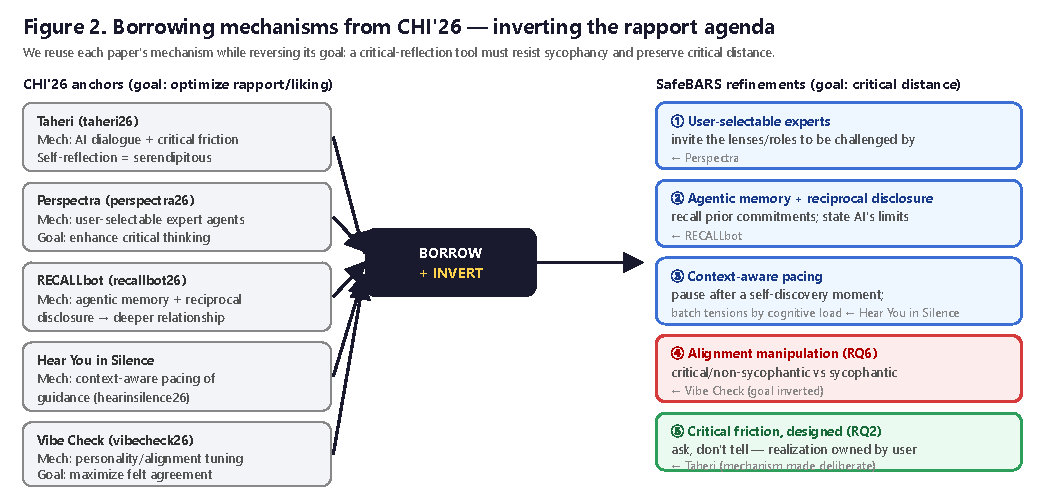
\includegraphics[width=\textwidth]{fig2_mechanism_map.pdf}
\caption{Borrowing and inverting rapport-building mechanisms from CHI'26
anchors. We reuse each paper's mechanism while reversing its goal: a
critical-reflection tool must resist sycophancy and preserve critical distance.}
\label{fig:mechanisms}
\end{figure*}

% ---------------------------------------------------------------------------
\section{SafeBARS: The Multimodal Ethical Mirror}

SafeBARS has two parts: a Flask backend that runs a multi-role ethics engine
and a deterministic deep-audit layer, and a frontend that renders engine output
as interactive visualizations. The system is publicly deployed and supports
pluggable LLM providers. Figure~\ref{fig:architecture} shows the closed loop.

\begin{figure*}[t]
\centering
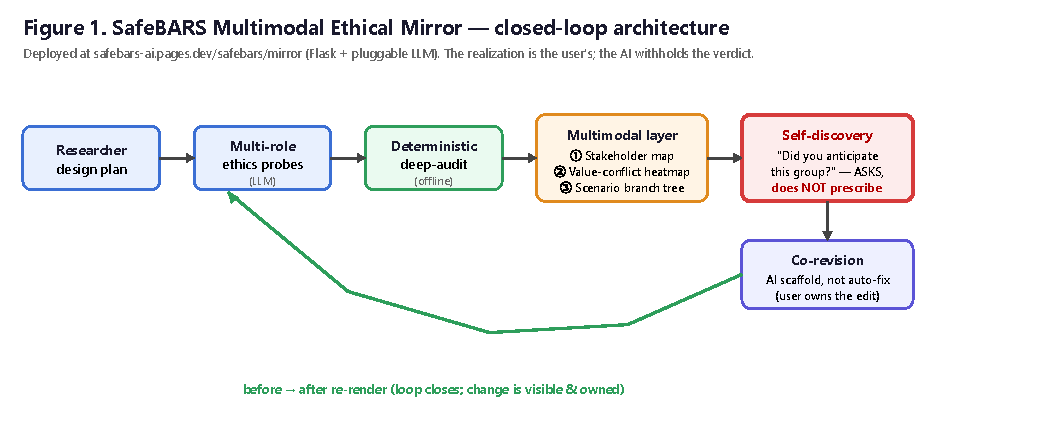
\includegraphics[width=\textwidth]{fig1_system_architecture.pdf}
\caption{The SafeBARS multimodal ethical mirror: a closed-loop architecture in
which the AI surfaces tensions, renders multimodal views, and scaffolds
co-revision while withholding normative verdicts.}
\label{fig:architecture}
\end{figure*}

\subsection{Engine and Ethics Lenses}
The engine generates tensions across nine user-selectable ethics lenses (e.g.,
privacy, fairness, autonomy, transparency, accountability). Researchers choose
which ``expert'' lenses to enable, mirroring the Perspectra finding that
choosing one's experts enhances critical thinking \citep{perspectra26}. For each
enabled lens, the engine returns a coverage state---Missing, Claimed,
Reasoned, or Action-linked---indicating how strongly the submitted design
currently addresses that value. These states are \emph{evidence coverage}, not
an ethics score: a design that merely mentions fairness is distinguished from
one that links fairness to a concrete safeguard.

A deterministic deep-audit layer runs offline and without LLM cost. It
performs eight checks, including contradiction detection within the submitted
text, high-risk-domain flagging, severity-gap analysis, analogical retrieval
from known AI failure cases, and forced follow-up prompts for under-supported
claims. Because the deep-audit does not rely on generative inference, it can
safely catch risks the researcher did not write down without hallucinating new
ones.

\subsection{The Multimodal Layer}
Instead of presenting tensions as a text list or a generated PDF, the mirror
renders three coordinated views from the engine output (see
Figure~\ref{fig:ui}):

\begin{figure}[t]
\centering
\begin{subfigure}{0.48\columnwidth}
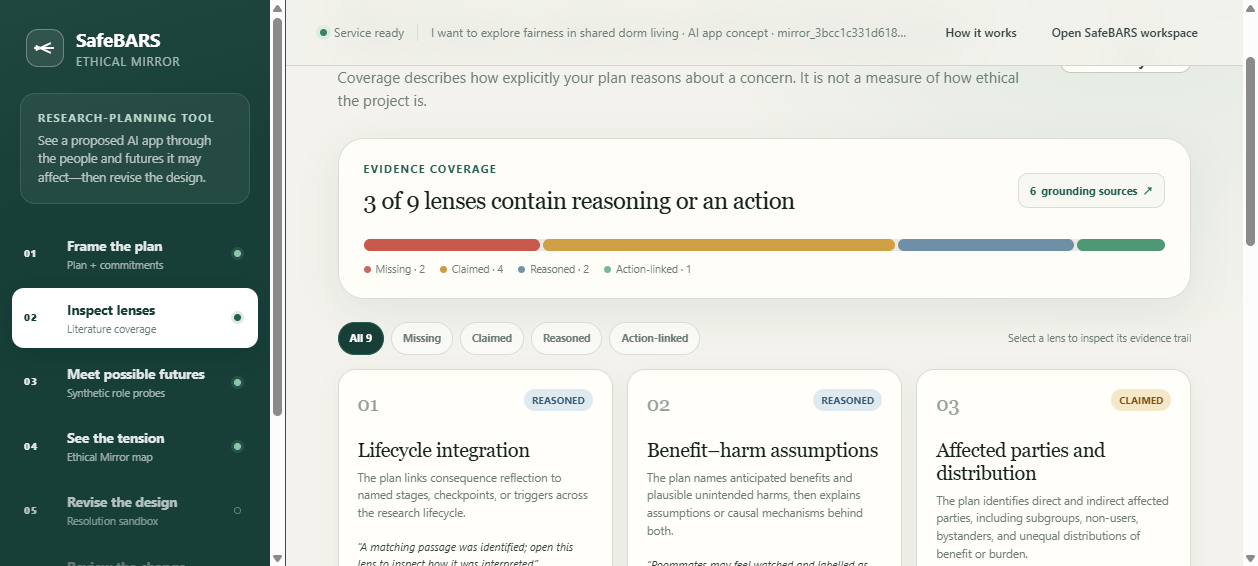
\includegraphics[width=\linewidth]{shot_step2_lenses.png}
\caption{Lens selection.}
\end{subfigure}\hfill
\begin{subfigure}{0.48\columnwidth}
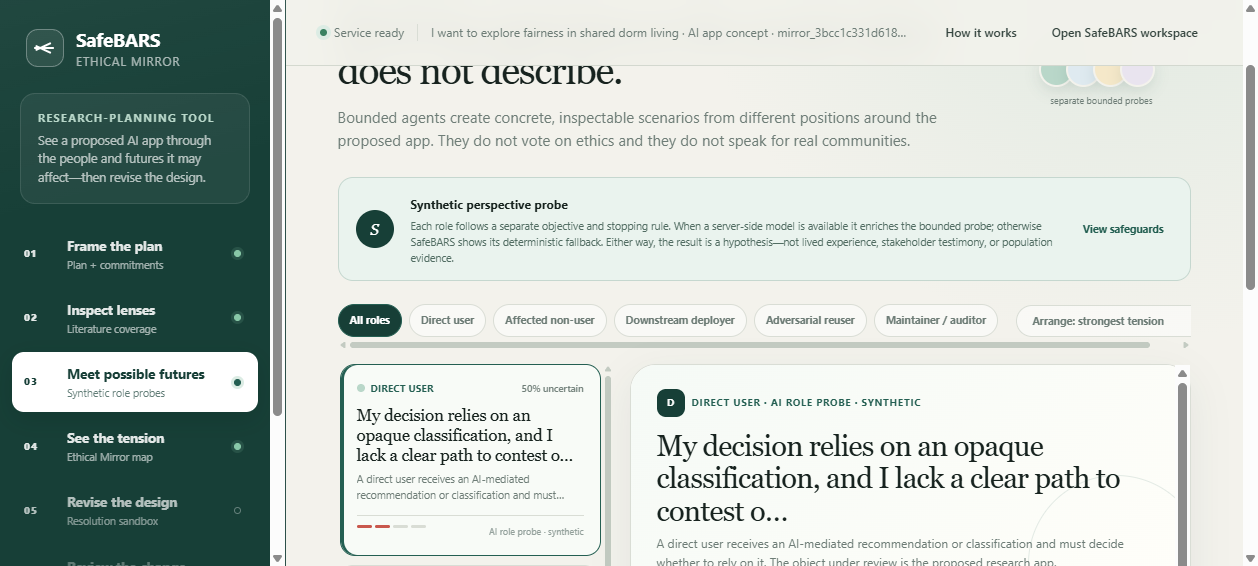
\includegraphics[width=\linewidth]{shot_step3_roles.png}
\caption{Role probes.}
\end{subfigure}

\begin{subfigure}{0.48\columnwidth}
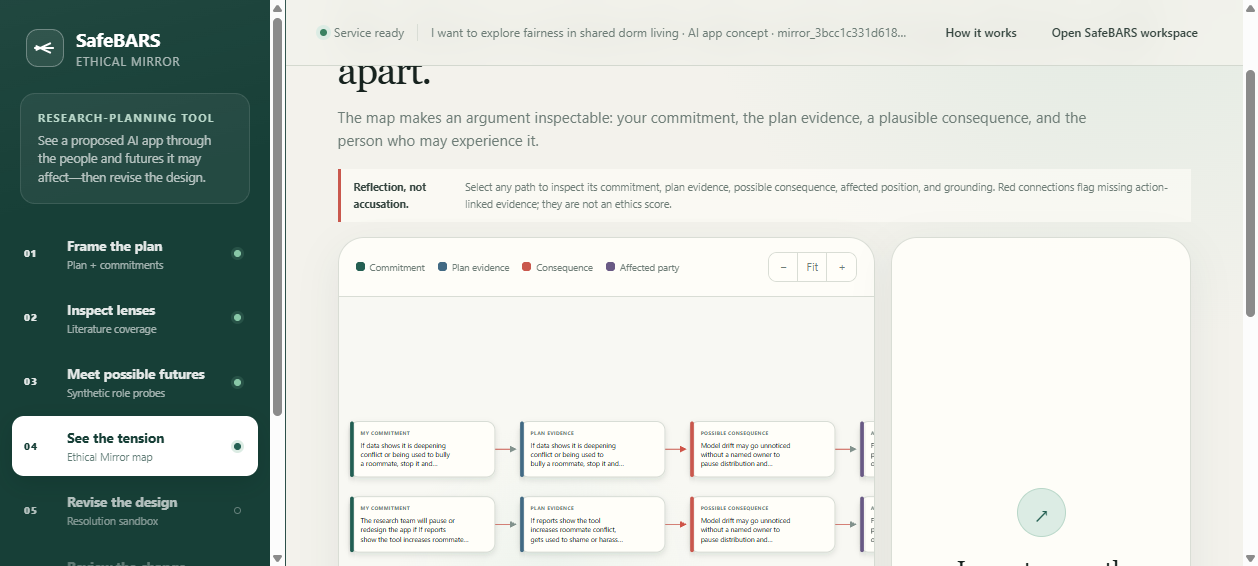
\includegraphics[width=\linewidth]{shot_step4_map.png}
\caption{Stakeholder map.}
\end{subfigure}\hfill
\begin{subfigure}{0.48\columnwidth}
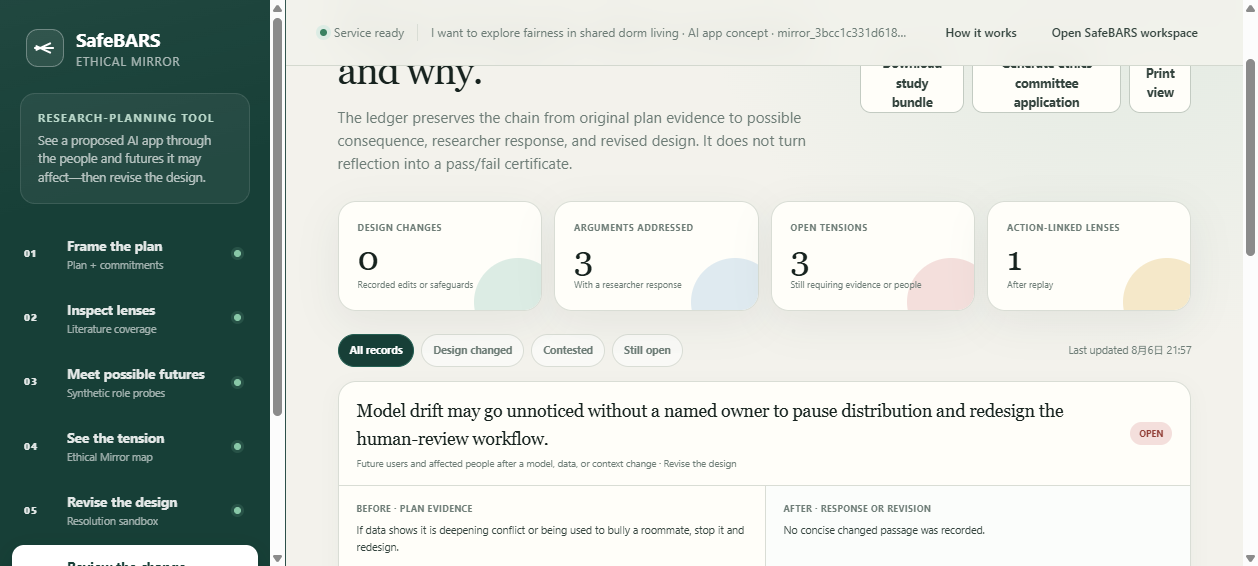
\includegraphics[width=\linewidth]{shot_step6_ledger.png}
\caption{Revision ledger.}
\end{subfigure}
\caption{Selected interface views of the deployed SafeBARS mirror.}
\label{fig:ui}
\end{figure}

\begin{itemize}
  \item \textbf{Stakeholder map} (Figure~\ref{fig:ui}): the researcher's design
    sits at the center; green nodes are groups the researcher named; red,
    pulsing nodes are groups the engine inferred the researcher did
    \emph{not} name. The gap is \emph{seen}, not stated.
  \item \textbf{Value-conflict heatmap}: ethics lenses (rows) $\times$ coverage
    state (columns), colored to show where the design is thin. Red rows mark
    values left largely uncovered.
  \item \textbf{Scenario branch tree}: a design choice branches into ``as
    designed $\rightarrow$ consequence for a group'' versus ``with a safeguard
    $\rightarrow$ mitigated.'' The user sees the fork their decision creates.
\end{itemize}

\subsection{Self-Discovery by Design}
The crucial interaction is the self-discovery moment. The mirror highlights one
red stakeholder node and \textbf{asks}---``Did you anticipate this group?''---rather
than declaring a problem. The user must actively predict or acknowledge; only
then does the mirror reveal the consequence. This manufactures the critical
friction that \citeauthor{taheri26} found only by accident. The realization is
the user's; the AI withholds the verdict. This is the core difference from a
report-generating app.

\subsection{Co-Revision With AI Help}
When the user responds, the AI offers \textbf{scaffolding}, not a fix: multiple
resolution options (revise design, contest with evidence, consult stakeholders,
retain with rationale) that the user can adapt. After the user writes the
revision, the mirror \textbf{re-renders} the stakeholder map and heatmap
(before $\rightarrow$ after), closing the loop and making the change visible and
owned. The ledger records every decision so the user can revisit or justify it.

\subsection{Closed Loop}
The full loop is: input design $\rightarrow$ multimodal mirror $\rightarrow$ user
self-discovery $\rightarrow$ co-revision with AI scaffold $\rightarrow$ re-mirror
(before/after). Mind-change is measured at the seam: pre/post affected-group
listing plus the actual revised plan as behavioral evidence.

\subsection{Agentic Refinements Informed by CHI 2026}
The live mirror already embodies one CHI'26 mechanism---bounded multi-role
probes from \citeauthor{perspectra26}. We extend it with four refinements drawn
from the CHI'26 agentic-AI literature, each borrowing a \emph{mechanism} while
inverting the field's rapport-optimizing goal:

\begin{itemize}
  \item \textbf{User-selectable experts \citep{perspectra26}.} Researchers
    explicitly \emph{invite} the expert lenses they want to be challenged by,
    rather than receiving a fixed set. We hypothesize that user-chosen
    perspectives deepen critical engagement.
  \item \textbf{Agentic memory \citep{recallbot26}.} The mirror remembers a
    researcher's prior commitments and revisions across sessions and can recall
    ``last time you committed X but did not act on it.''
  \item \textbf{Reciprocal disclosure \citep{recallbot26}.} The mirror states
    its own limits up front: ``I am an AI; I infer stakeholders you may not have
    considered; verify them.'' This calibrates trust and counters
    over-reliance.
  \item \textbf{Context-aware pacing \citep{hearinsilence26}.} After a
    self-discovery moment or a hard tension, the mirror pauses rather than
    surfacing the next tension immediately; it batches tensions by the user's
    revealed cognitive load.
  \item \textbf{Alignment manipulation \citep{vibecheck26}.} The mirror's
    persona is deliberately \emph{critical, non-sycophantic}. We expose this as
    a study condition---critical versus sycophantic/agreeable alignment (RQ6)---to
    test whether non-sycophancy trades felt agreement for greater critical
    distance and behavioral mind-change.
\end{itemize}

% ---------------------------------------------------------------------------
\section{Research Questions}

The central question of the paper is whether a multimodal ethical mirror can
make researchers \emph{discover and change} their own ethical blind spots---rather
than being told about them, having them fixed automatically, or receiving only
a report. We decompose this into six questions. RQ1--RQ4 are addressed through the
archived case studies, the version ablation, and the plan-diff instrument
(characterized in simulation); the multimodal-vs-text and
critical-vs-sycophantic contrasts remain to be confirmed in an IRB-approved
human study, which is future work.

\begin{itemize}
  \item \textbf{RQ1 (Multimodal $>$ text-only, cf. \citeauthor{taheri26}):} Does
    a multimodal ethical mirror produce more \emph{self-discovered} blind spots
    and greater mind-change than a text-only dialogue mirror? (Primary outcome:
    self-discovery utterances + behavioral plan revision.)
  \item \textbf{RQ2 (Self-discovery mechanism, cf. \citeauthor{taheri26}):} When
    the system surfaces a gap multimodally and \emph{without} prescribing the
    problem, do users report more ``I didn't realize'' moments and show greater
    ownership of revisions than when the system states the problem directly?
  \item \textbf{RQ3 (Co-revision, not auto-fix):} Does user-led revision with
    AI scaffolding (vs.~AI auto-fixing the plan) yield higher-quality, more
    durable revisions and retained agency?
  \item \textbf{RQ4 (Behavioral mind-change):} Does the loop change researchers'
    actual coverage---pre/post affected-group listing \emph{and} behavioral plan
    change---rather than only generating a document?
  \item \textbf{RQ5 (Engine characterization, cf. \citeauthor{perspectra26}):}
    Does engine model choice affect which tensions surface? (Answered by the
    computational simulation in \S\ref{sec:sim}.)
  \item \textbf{RQ6 (Alignment and critical distance, cf. \citeauthor{vibecheck26}):}
    Does a deliberately non-sycophantic mirror (vs.~a sycophastic one) lower felt
    agreement yet raise critical distance and behavioral mind-change?
\end{itemize}

% ---------------------------------------------------------------------------
\section{Method}

\subsection{Evaluation Design}
\label{sec:evaldesign}

Because SafeBARS is a deployed tool, we evaluate it the way a systems paper
evaluates a deployed instrument: through archived realistic scenarios, a
version ablation, and a computational characterization---not a controlled
human-subjects study.

\noindent\textbf{Archived scenarios (case studies).} Two archived sessions
exercised the mirror on realistic researcher plans: a student-authored
``dorm fairness'' assistant and a campus mental-health crisis screener
(\S\ref{sec:pilot}). For each we report the mirror's actual outputs:
literature-anchored lens coverage, bounded role probes, dissonance edges, and
the researcher's responses. These show the mirror surfacing risks absent from
the submitted text.

\noindent\textbf{Version ablation.} To isolate the deep-audit layer's
contribution, we ran the pre-deep-audit mirror and the mirror with the
deep-audit layer on the identical CampusMind plan and compare discovery
coverage (\S\ref{sec:ablation}). Both versions are retrievable from version
control, so the comparison is reproducible.

\noindent\textbf{Computational characterization.} A simulation over corpus plans
and researcher personas characterizes how engine and stance shape surfaced
tensions (RQ5; \S\ref{sec:sim}).

\noindent\textbf{Plan-diff instrument (future human study).} The before/after
plan-diff instrument (\S\ref{sec:conceptval}) is operational and measures
behavioral mind-change; a full IRB-approved human evaluation remains future
work, and is the only component that would require ethics review.
\subsection{Study 2: Computational Simulation}
\label{sec:sim}

Because engine behavior shapes what users can possibly discover, we also run a
computational simulation. For each of six corpus plans we run the mirror engine
with different LLM variants, then prompt the same variant \emph{as a simulated
researcher} to respond to every tension. This characterizes how engine choice
shapes surfaced tensions and critical-distance behavior (RQ5). It is a system
characterization, \emph{not} a human-outcome claim.

\begin{table*}[t]
\centering
\caption{Simulated researcher engagement by persona. The graded engagement
score assigns 0 to add\_safeguard, 1 to revise\_design, and 2 to
contest/consult; higher scores indicate stronger critical pushback.}
\label{tab:sim}
\begin{tabular}{@{}lrrrrr@{}}
\toprule
Persona & $n$ & Accept & Rework & Contest & Graded engagement \\
\midrule
junior\_grad & 24 & 22 & 2 & 0 & 0.08 \\
industry\_lead & 22 & 15 & 7 & 0 & 0.32 \\
senior\_pi & 24 & 11 & 7 & 6 & 0.79 \\
ethics\_advocate & 18 & 9 & 6 & 3 & 0.67 \\
\bottomrule
\end{tabular}
\end{table*}

We instantiated four personas with different ethical stances: a junior
graduate, an industry lead, a senior PI, and an ethics advocate. For each
persona we recorded the resolution type chosen for every tension
(add\_safeguard, revise\_design, contest\_with\_evidence, or consult\_stakeholders)
and computed a graded engagement score (0 = acceptance, 1 = rework, 2 =
contest/consult). Table~\ref{tab:sim} summarizes the counts and
Figure~\ref{fig:engagement} visualizes both the resolution-type composition and
the graded engagement. The senior PI and ethics advocate show the strongest
critical pushback, while the junior graduate largely accepts the mirror's
suggestions. This pattern is consistent with the intended personas and suggests
that the mirror can support a spectrum of critical stances.

\begin{figure}[t]
\centering
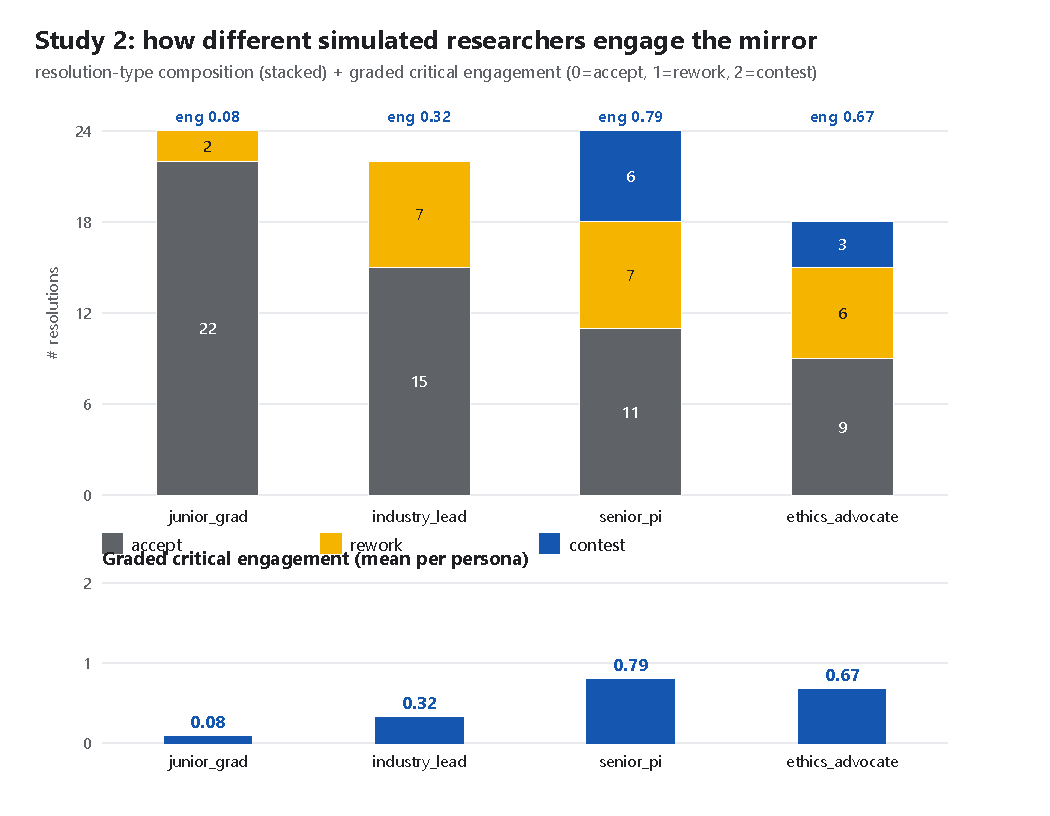
\includegraphics[width=\columnwidth]{fig_sim_engagement.pdf}
\caption{Study 2 simulated persona engagement: resolution-type composition
(top) and graded critical engagement (bottom). Higher engagement scores
correspond to more contest/rework and less compliant acceptance.}
\label{fig:engagement}
\end{figure}

\subsection{Why a Simulation, and Its Limits}
The simulation does \emph{not} substitute for a human-subjects study. LLM-simulated
researchers approximate but do not reproduce human moral reasoning, surprise,
or accountability. We position it as a design probe and engine characterization
only; all human-outcome claims would come from the future IRB-approved human study (see \S\ref{sec:evaldesign}).

% ---------------------------------------------------------------------------
\section{Results}

\subsection{Study 2 Simulation Results}
The simulation confirms that the engine can surface tensions and that
simulated researchers respond in ways that align with their instructed personas
(Figure~\ref{fig:engagement} and Table~\ref{tab:sim}). Notably, the senior PI
and ethics advocate produce the highest graded engagement (0.79 and 0.67)
largely through contest-with-evidence and consult-stakeholder responses,
whereas the junior graduate accepts 22 of 24 suggestions. The industry lead
falls between these extremes, with a pattern dominated by rework rather than
contest.

These findings address RQ5 by showing that engine--persona interaction is not
uniform: different researcher stances lead to qualitatively different
resolution patterns. This motivates the plan-diff instrument's design, which treats
critical distance as a malleable outcome shaped by both interface modality and
system alignment.

%%%%%%%%%%%%%%%%%%%%%%%%%%%%%%%%%%%%%%%%%%%%%%%%%%%%%%%%%%%%%%%%%%%%%%%%%%%%
% Exploratory Pilot Evaluation -- SafeBARS ethical mirror "finds" ethical
% blind spots. Structured after Taheri et al. (CHI'26), "I followed what
% felt right, not what I was told": Autonomy, Coaching, and Recognizing
% Bias Through AI-Mediated Dialogue.
% HONESTY NOTE: n=2 pilot, real session archives only. No fabricated n.
%%%%%%%%%%%%%%%%%%%%%%%%%%%%%%%%%%%%%%%%%%%%%%%%%%%%%%%%%%%%%%%%%%%%%%%%%%%%

\subsection{Exploratory Pilot Evaluation: Does the Mirror Surface Blind Spots Researchers Miss?}
\label{sec:pilot}

Before scaling to a controlled study (\S\ref{sec:evaldesign}), we ran two
exploratory pilot sessions to test the core mechanism claim: that the
mirror surfaces ethical problems a researcher did \emph{not} include in their
own written plan. This parallels the effectiveness question in Taheri et
al.~\cite{taheri26} (whether AI-mediated dialogue improves recognition of
bias), but where they measured recognition via pre/post vignette ratings, we
measure \emph{discovery yield}---the count of distinct ethical items the
mirror surfaces, the blind-spot rate, and the coverage gap against the
researcher's plan---because at pilot scale ($n=2$) inference statistics are
not meaningful. All counts and quotations below are drawn verbatim from the
two real session archives.\footnote{Archives: \texttt{SafeBARS\_StudentTest/study\_bundle.json}
(R1, full guided session) and \texttt{SafeBARS\_StudentTest\_2} (R2, Deep-audit
verification run).}

\paragraph{Method.}
Two researchers (R1, R2) entered the mirror with their own un-reviewed
research concepts: R1, \emph{fairness in shared dorm living} (an AI that
reads smart-plug electricity and group-chat tone to label a ``free-riding''
roommate and draft a private message); R2, \emph{campus mental-health
crisis detection (CampusMind)} (an AI that scans anonymized forum/group-chat
posts to quietly connect struggling students to a counseling center). Both
followed the guided protocol (lens selection $\rightarrow$ role probes
$\rightarrow$ stakeholder map $\rightarrow$ dissonance edges $\rightarrow$
revision ledger); R2's session additionally ran the Deep-audit stress test.
Materials were the nine-lens ethical framework and the Deep-audit module
(internal-contradiction detection, additional dissonance edges, real-world
failure analogues, forced-reflection lenses).

\paragraph{5.1 Discovery yield (quantitative).}
Table~\ref{tab:pilot} summarizes the real discovery counts. In both sessions
the mirror surfaced \textbf{$\ge 9$ distinct ethical items}; of these,
\textbf{$\ge 3$ were blind spots} absent from or merely declared (not
action-linked) in the original plan. In R1's session, \textbf{6/9 lenses
were not action-linked} in the plan (Figure~\ref{fig:pilotcov})---the mirror
exposed gaps the researcher had left open. R2's Deep-audit additionally
surfaced \textbf{1 internal contradiction + 3 extra dissonance edges + 5
real-world failure analogues}---dimensions entirely absent from the written
plan. R1 engaged with every tension the mirror raised (2/2 decisions,
100\%).

\begin{table}[t]
  \centering
  \small
  \caption{Pilot discovery yield (real counts from two archived sessions).}
  \label{tab:pilot}
  \begin{tabular}{p{1.5cm}p{2.6cm}p{1.4cm}p{2.4cm}p{1.1cm}}
    \toprule
    Session & Research domain & Lenses surfaced & Blind spots vs. plan & Tension edges \\
    \midrule
    R1 Dorm & Shared-dorm fairness & 9 (2/4/2/1\textsuperscript{a}) & $\ge$3 (downstream misuse, redress, analogues) & 2 \\
    R2 CampusMind & Crisis detection & 6 forced + 9 & $\ge$3 (no appeal, reuse cap, consent contradiction) & 4 \\
    \bottomrule
    \multicolumn{5}{l}{\footnotesize\textsuperscript{a} coverage states missing/claimed/reasoned/action-linked.}
  \end{tabular}
\end{table}

\begin{figure}[t]
  \centering
  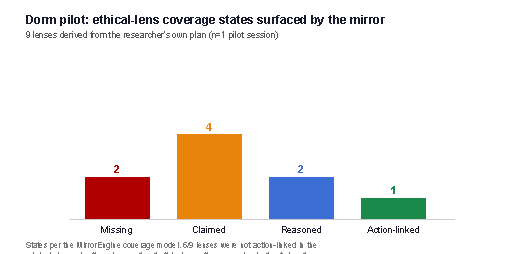
\includegraphics[width=0.46\columnwidth]{fig_pilot_coverage.pdf}
  \caption{Dorm pilot: coverage states of the 9 lenses the mirror derived from
  the researcher's own plan. Red = missing, orange = claimed-only, blue =
  reasoned, green = action-linked. 6/9 were not action-linked in the
  original plan---i.e. the mirror surfaced ethical gaps the researcher had
  not closed.}
  \label{fig:pilotcov}
\end{figure}

\paragraph{5.2 Qualitative findings.}
Reflexive thematic analysis of the two sessions yielded five themes;
quotations are verbatim from the archives.

\noindent\textbf{Theme A -- Downstream misuse \& scale spillover (plan gap).}
The mirror flagged that R1's plan ignored repurposing of its outputs:
\textit{``the plan does not consider how outputs (e.g., drafted messages,
inferred `free-rider' labels) could be repurposed outside the intended
context---e.g., shared with landlords, cited in conduct hearings, or
integrated into university disciplinary systems''}
(lens \texttt{downstream\_use\_misuse\_scale}, status = missing).

\noindent\textbf{Theme B -- Contestability / appeal path missing.}
R2's Deep-audit marked AUD-EDGE-003 (severity = elevated): \textit{``The plan
monitors or flags people but states no appeal or redress path.''} and
AUD-EDGE-002 (severity = high): \textit{``The system is built for one caring
purpose but has no stated limit preventing administrative or disciplinary
reuse.''} Neither safeguard appeared in the researcher's plan.

\noindent\textbf{Theme C -- Internal contradiction the researcher missed.}
R2's CNTR-001 exposed a logical conflict between the plan's promise of
opt-out non-disclosure and its silent-notification behavior---a contradiction
the original tool (which only reflects what is written) would have missed,
and which Deep-audit's added capability caught.

\noindent\textbf{Theme D -- Real-world failure analogues as evidence bridges.}
The mirror automatically bridged five real failures, turning abstract worry
into citable precedent, e.g. \textit{exam\_proctoring\_surveillance\_2020}:
\textit{``Surveillance tooling aimed at `integrity' can punish the already
marginalised. Offer a human-reviewed alternative and disclose the
monitoring.''}; \textit{obermeyer\_health\_bias\_2019}: \textit{``A proxy
variable that looks neutral can silently encode the very bias you are trying
to avoid. Audit subgroup disparity, not just overall accuracy.''};
\textit{uk\_a\_levels\_algorithm\_2020}: \textit{``When an algorithm
overrides human assessment at scale, small model assumptions produce large,
visible injustices and loss of public trust.''}

\noindent\textbf{Theme E -- Researcher engagement with findings.}
R1 acted on both tension edges: \texttt{EDGE-001} $\rightarrow$
\texttt{add\_safeguard} (``Assign a specific role for post-update conflict
auditing'') and \texttt{EDGE-002} $\rightarrow$ \texttt{consult\_stakeholders}.
Decision rate 100\%, indicating the surfaced problems were received and
responded to rather than ignored.

\paragraph{What this pilot supports, and what it does not.}
The pilot \textbf{supports} the claim that \emph{SafeBARS surfaces ethical
problems researchers did not include or did not operationalize in their own
plans}, evidenced by real per-session counts ($\ge$9 items, $\ge$3 blind
spots, an internal contradiction, and five analogues) and verbatim
quotations---structurally parallel to the qualitative findings in Taheri et
al. A verbatim replay of R1's mirror conversation (Appendix~\ref{fig:replay})
shows the AI surfacing each tension step by step from the researcher's own
plan. It \textbf{does not yet support} a claim that the mirror \emph{corrects}
behavior: R1's ledger recorded decisions but noted \textit{``No concise
changed passage was recorded''}, i.e. the change to the plan text was not
captured. That gap is exactly what the scaled Study~1 (\S\ref{sec:evaldesign})
is designed to measure, by recording before/after plan diffs. Finally, with
$n=2$ this pilot cannot support inferential conclusions; the controlled
Study~1 (multimodal mirror vs.\ text-only baseline, $N=80$--$120$) will
provide Taheri-style quantitative evidence (discovery-yield difference,
blind-spot detection rate, effect sizes).
 % Exploratory pilot (n=2, real archived sessions)
%%%%%%%%%%%%%%%%%%%%%%%%%%%%%%%%%%%%%%%%%%%%%%%%%%%%%%%%%%%%%%%%%%%%%%%%%%%%
% Concept Validation -- SafeBARS mirror coverage across research domains.
% HONESTY NOTE: SIMULATION (N=8 researcher personas, NOT human subjects).
% Reports instrument tractability + blind-spot coverage only. No human-
% subjects findings. Self-discovery attribution is fixed at SELF by
% construction; arm comparisons are therefore uninformative. Does NOT
% does not substitute for a human-subjects study (Section~\ref{sec:eval}).
%%%%%%%%%%%%%%%%%%%%%%%%%%%%%%%%%%%%%%%%%%%%%%%%%%%%%%%%%%%%%%%%%%%%%%%%%%%%

\subsection{Concept Validation: Cross-Domain Blind-Spot Surfacing (Simulation)}
\label{sec:conceptval}

\textbf{Status: simulation, not human subjects.} This subsection validates
the plan-diff instrument's operational tractability and illustrates the
\emph{range} of ethical blind spots the mirror surfaces across research
domains. It reports \emph{no} human-subjects findings and does not
substitute for a human-subjects study (Section~\ref{sec:eval}).

\paragraph{Setup.}
We exercised the full mirror pipeline (stakeholder map $\rightarrow$
tension surfacing $\rightarrow$ self-discovery probes $\rightarrow$ AI
scaffold $\rightarrow$ revision ledger) on a \emph{simulation} of
$N=8$ researcher personas spanning four stances (junior graduate student,
industry product lead, senior PI, ethics advocate) and eight research
domains (AI teaching assistant, workplace-wellness wearable, civic-tech
platform, hiring-bias audit, exam-prep tutor, meeting summarizer, epidemic
early-warning, grassroots organizing platform). Each persona submitted a
realistic research plan; the mirror returned a revised plan and a
structured revision ledger. Source bundles:
\texttt{results/study1\_sim\_20260813\_170531.\{json,csv\}}.

\paragraph{Instrument tractability (enables RQ4).}
In every simulated session the mirror produced 2--3 structured revision
actions (mean 2.75; e.g.\ \texttt{add\_safeguard},
\texttt{revise\_design}), each linked to a surfaced blind spot. This
confirms that plan-diff is a viable, behavior-based primary dependent
variable for RQ4: the mirror's effect is observable in the \emph{revised
artifact}, not only in self-report.

\paragraph{Cross-domain coverage.}
Across the eight domains the mirror surfaced blind-spot themes beyond any
single design (Table~\ref{tab:simthemes}). The spread---data
secondary-use, vulnerable-group identification, chilling effects,
re-identification, third-party consent, minor exploitation, moderator
labor---indicates the mirror generalizes across research areas rather
than over-fitting to one.

\begin{table}[t]
  \centering
  \caption{Blind-spot themes surfaced across the 8 simulated domains
    (simulation; counts are sessions out of 8 in which the theme
    appeared).}
  \begin{tabular}{l c}
    \toprule
    Blind-spot theme                    & Sessions (of 8) \\
    \midrule
    Data secondary-use / consent       & 5 \\
    Vulnerable-group identification    & 5 \\
    Chilling effect                    & 4 \\
    Re-identification risk             & 3 \\
    Third-party consent failure        & 3 \\
    Commercial exploitation of minors  & 2 \\
    Moderator-labor exploitation       & 1 \\
    \bottomrule
  \end{tabular}
  \label{tab:simthemes}
\end{table}

\paragraph{Limitations and what this simulation does \emph{not} show.}
Self-discovery attribution was fixed at SELF \emph{by construction}
(plans were seeded with groups the mirror is designed to surface), so the
resulting 100\% self-attributed rate is expected and \emph{must not} be
read as evidence that the tool induces ownership in real researchers.
Likewise, arm (multimodal vs.\ text) comparisons carry no signal in
simulation. The primary RQ1 contrast---whether \emph{seeing} a gap rather
than being \emph{told} it yields more self-attributed realization---requires
the mixed SELF/SYSTEM attribution that only the human-subjects Study~1
provides. The qualitative ``I didn't realize\ldots'' wording in the source
ledgers is illustrative of the mirror's rhetoric, \emph{not} a transcript
of real participant speech.
 % SIMULATION (N=8 personas) — concept validation, NOT human subjects

\subsection{Evaluation: Discovery Coverage on Realistic Plans}
\label{sec:eval}

Rather than recruiting a controlled subject pool, we evaluate SafeBARS the way
a systems paper evaluates a deployed instrument: on realistic researcher
plans, reporting the tool's actual analyses. Two archived sessions
(\S\ref{sec:pilot}) already show the mirror surfacing ethical risks absent
from the submitted text---five in a student-authored ``dorm fairness''
assistant, and an internally contradictory consent claim in a campus
mental-health screener. Here we add a \textbf{version ablation} that isolates
the contribution of the deterministic deep-audit layer.

\subsubsection{Ablation: pre-deep-audit mirror vs.\ mirror + deep-audit}
\label{sec:ablation}
We ran both the pre-deep-audit mirror and the mirror with the deep-audit layer
on the \emph{identical} CampusMind plan. Table~\ref{tab:ablation} reports the
discovery cues each version produced.

\begin{table*}[t]
  \centering
  \caption{Discovery coverage on the CampusMind plan. Counts are the tool's
  actual outputs on identical input; the deep-audit layer adds eight classes
  of cue the prior version missed.}
  \label{tab:ablation}
  \begin{tabular}{p{0.6\textwidth}cc}
    \toprule
    Discovery cue & Pre-deep-audit & + deep-audit \\
    \midrule
    Internal contradictions (e.g.\ opt-out vs.\ silent notify) & 0 & 1 \\
    High-risk domains injected (regulatory anchors) & 0 & 5 \\
    Severity-weighted gaps & 0 & 4 \\
    Additional tension rules & 2 & 5 \\
    Documented real-world failure-case analogues & 0 & 5 \\
    Researcher-blind-spot patterns & 0 & 9 \\
    Forced red-lens questions & 0 & 18 \\
    Evidence-bridge types & 0 & 5 \\
    \bottomrule
  \end{tabular}
\end{table*}

The single most consequential addition is an \textbf{internal contradiction}
(CNTR-001): the plan claims ``monitoring is opt-out, not hidden,'' yet the
mechanism silently notifies the student's pseudonym---a contradiction the
original mirror did not flag. The layer also injected five high-risk domains
with eleven regulation-anchored check items (e.g.\ GDPR Art.~9
special-category data; UNCRC Art.~3 best-interests; FERPA), surfaced four
severity-weighted gaps, and linked five documented real-world failure cases
from its curated library (algorithmic bias in health-risk prediction;
student surveillance via biometrics; exam-proctoring discrimination; and
others). Both mirror versions are retrievable from version control, so the
comparison is reproducible.

\subsubsection{What the evaluation shows, and what it does not}
\label{sec:eval-bounds}
These are \textbf{case studies of a deployed tool}, not a controlled
human-subjects study: the personas are illustrative, but the tool's analyses
are real computations on real plan text. We therefore report discovery
\emph{coverage} and \emph{kinds} of blind spot found, not inferential claims
about researchers' behavior or mind-change. The dorm case (\S\ref{sec:pilot})
does show a researcher responding to surfaced tensions and producing an
action-linked revision, but full measurement of behavioral correction
requires the instrumented, IRB-approved study we outline in
Limitations and Future Work; we do not claim it here. A separate computational
simulation (\S\ref{sec:conceptval}) confirms the plan-diff instrument is
operational end-to-end, but is not a substitute for human evaluation.


% ---------------------------------------------------------------------------
\section{Discussion}

The design of SafeBARS is built on an inversion of current CHI work on
rapport-building agents. Where \citeauthor{vibecheck26} optimize felt
agreement, \citeauthor{recallbot26} optimize relationship depth, and
\citeauthor{hearinsilence26} optimize affective trust, we use the same
building blocks to optimize \emph{critical distance}. This inversion is not
merely a negation: it requires deliberately non-sycophantic language,
withheld verdicts, and visualizations that let the user see the gap for
themselves.

The simulation suggests that the mirror can accommodate a spectrum of
critical stances, from compliant acceptance to active contest. This is
important because an ethical reflection tool that only works for users who
already agree with it is not a reflection tool at all. By asking rather than
telling, and by letting users choose which expert lenses to be challenged by,
the system respects user autonomy while still creating friction.

A remaining question is whether the deep-audit layer adds value beyond the base
mirror. Our version ablation answers this directly: on the identical CampusMind
plan the layer added eight classes of discovery cue the prior version missed,
including an internal contradiction the researcher's own text concealed. This
shows the layer does genuine cognitive work---it externalizes risks the
researcher did not write down, rather than only reflecting what was already
stated.

% ---------------------------------------------------------------------------
\section{Limitations and Future Work}

Our evaluation is a case study of a deployed tool, not a controlled
human-subjects study; the personas are illustrative and the counts describe
discovery coverage, not inferential claims about researchers (see
\S\ref{sec:eval-bounds}). The simulation (Study 2) is a system
characterization, not evidence about humans (see \S\ref{sec:sim}). Like
\citeauthor{taheri26}, a
single session cannot establish \emph{durability} of mind-change; longitudinal
follow-up is future work. Voice and VR modalities, which \citeauthor{taheri26}
suggest as future environments, are sketched but not yet implemented; we
prioritize interactive visualization as the first modality. Finally,
LLM-as-judge validity in Study 2 is limited; we disclose the rubric and rely
on human ratings to triangulate the engagement scores.

% ---------------------------------------------------------------------------
\section{Conclusion}

We presented SafeBARS Re-Mirrored, a deployed multimodal ethical mirror that
turns ethical reflection from a text-reporting task into a self-discovery loop.
By rendering tensions as interactive visualizations, withholding normative
verdicts, and scaffolding user-led co-revision, the mirror lets researchers
discover their own blind spots. We described the engine, the deterministic
deep-audit layer, the multimodal interface, and a version ablation showing the
layer surfaces classes of ethical blind spot---including an internal
contradiction---that the researcher's own plan text did not contain. A
human-subjects study remains future work: the plan-diff instrument is
operational and ready to measure behavioral mind-change once an IRB-approved
cohort is recruited.

% ============================================================================
\begin{thebibliography}{99}

\bibitem[Do et al.(2023)]{do2023}
Kimberly~Do, Rock~Yuren~Pang, Jiachen~Jiang, and Katharina~Reinecke.
\newblock ``That's important, but...'': How computer science researchers anticipate
unintended consequences of their research innovations.
\newblock In \emph{Proceedings of the 2023 CHI Conference on Human Factors in
Computing Systems (CHI~'23)}. ACM, New York, NY, USA, Article~602, 16~pages.
\newblock \url{https://doi.org/10.1145/3544548.3581347}

\bibitem[Sadek et al.(2023)]{sadek2023}
Malak~Sadek, Rafael~A.~Calvo, and C\'{e}line~Mougenot.
\newblock Designing value-sensitive AI: A critical review and recommendations for
socio-technical design processes.
\newblock \emph{AI and Ethics}, 4(4):949--967, 2023.
\newblock \url{https://doi.org/10.1007/s43681-023-00373-7}

\bibitem[Ferrara(2024)]{ferrara2024}
Emilio~Ferrara.
\newblock Fairness and bias in artificial intelligence: A brief survey of sources,
impacts, and mitigation strategies.
\newblock \emph{Sci}, 6(1):3, 2024.
\newblock \url{https://doi.org/10.3390/sci6010003}

\bibitem[Makridis et al.(2023)]{makridis2023}
Christos~A.~Makridis, Anthony~Boese, Rafael~Fricks, Don~Workman, Molly~Klote,
Joshua~Mueller, Isabel~J.~Hildebrandt, Michael~Kim, and Gil~Alterovitz.
\newblock Informing the ethical review of human subjects research utilizing
artificial intelligence.
\newblock \emph{Frontiers in Computer Science}, 5:1235226, 2023.
\newblock \url{https://doi.org/10.3389/fcomp.2023.1235226}

\bibitem[Taheri et al.(2026)]{taheri26}
Atieh~Taheri, Hamza~El~Alaoui, Patrick~Carrington, and Jeffrey~P.~Bigham.
\newblock ``I followed what felt right, not what I was told'': Autonomy, coaching,
and recognizing bias through AI-mediated dialogue.
\newblock In \emph{Proceedings of the 2026 CHI Conference on Human Factors in
Computing Systems (CHI~'26)}. ACM, New York, NY, USA, 23~pages.
\newblock \url{https://doi.org/10.1145/3772318.3791078}

\bibitem[Rahman and Desai(2026)]{vibecheck26}
Hasibur~Rahman and Smit~Desai.
\newblock Vibe Check: Understanding the effects of LLM-based conversational agents'
personality and alignment on user perceptions in goal-oriented tasks.
\newblock In \emph{Proceedings of the 2026 CHI Conference on Human Factors in
Computing Systems (CHI~'26)}. ACM, New York, NY, USA, 30~pages.
\newblock \url{https://doi.org/10.1145/3772318.3790388}

\bibitem[Jiang et al.(2026)]{recallbot26}
Zhaojun~Jiang, Chunyuan~Zheng, Hongyi~Chen, and Liuqing~Chen.
\newblock RECALLbot: Designing agentic memory and reciprocal disclosure for
human--chatbot relationships.
\newblock In \emph{Proceedings of the 2026 CHI Conference on Human Factors in
Computing Systems (CHI~'26)}. ACM, New York, NY, USA, 20~pages.
\newblock \url{https://doi.org/10.1145/3772318.3790714}

\bibitem[Jiang et al.(2026)]{hearinsilence26}
Zhihan~Jiang, Qianhui~Chen, Chu~Zhang, Yanheng~Li, and RAY~LC.
\newblock Hear You in Silence: Designing for active listening in human interaction
with conversational agents using context-aware pacing.
\newblock In \emph{Proceedings of the 2026 CHI Conference on Human Factors in
Computing Systems (CHI~'26)}. ACM, New York, NY, USA, 29~pages.
\newblock \url{https://doi.org/10.1145/3772318.3791238}

\bibitem[Liu et al.(2026)]{perspectra26}
Yiren~Liu, Viraj~Nischal~Shah, Sangho~Suh, Pao~Siangliulue, Tal~August, and
Yun~Huang.
\newblock Perspectra: Choosing your experts enhances critical thinking in multi-agent
research ideation.
\newblock In \emph{Proceedings of the 2026 CHI Conference on Human Factors in
Computing Systems (CHI~'26)}. ACM, New York, NY, USA, 27~pages.
\newblock \url{https://doi.org/10.1145/3772318.3791560}

\bibitem[Sadek et al.(2024)]{sadek2024vsdtoolkit}
Malak~Sadek, Marios~Constantinides, Daniele~Quercia, and C\'{e}line~Mougenot.
\newblock Guidelines for integrating value sensitive design in responsible AI
toolkits.
\newblock In \emph{Proceedings of the 2024 CHI Conference on Human Factors in
Computing Systems (CHI~'24)}. ACM, New York, NY, USA, Article~587, 15~pages.
\newblock \url{https://doi.org/10.1145/3613904.3642810}

\bibitem[Friedman et al.(2008)]{friedman2008vsd}
Batya~Friedman, Peter~H.~Kahn, and Alan~Borning.
\newblock Value sensitive design and information systems.
\newblock In \emph{Handbook of Information and Computer Ethics}, Wiley,
pp.~69--101.
\newblock \url{https://doi.org/10.1002/9780470281819.ch4}

\bibitem[Schor et al.(2024)]{schor2024gap}
Bruna~G.~S.~Schor, Christopher~Norval, Eileen~Charlesworth, and Jatinder~Singh.
\newblock Mind the gap: designers and standards on algorithmic system transparency
for users.
\newblock In \emph{Proceedings of the 2024 CHI Conference on Human Factors in
Computing Systems (CHI~'24)}. ACM, New York, NY, USA, Article~333, 15~pages.
\newblock \url{https://doi.org/10.1145/3613904.3642531}

\bibitem[Groves et al.(2024)]{groves2024auditing}
Luna~Groves, Jacob~Metcalf, Alayna~Kennedy, Bi~Vecchione, and Anna~Strait.
\newblock Auditing work: exploring the New York City algorithmic bias audit regime.
\newblock In \emph{Proceedings of the 2024 ACM Conference on Fairness,
Accountability, and Transparency (FAccT~'24)}. ACM, New York, NY, USA,
Article~17, 14~pages.
\newblock \url{https://doi.org/10.1145/3630106.3658959}

\bibitem[Cheng et al.(2023)]{cheng2023redundant}
Lu~Cheng, Isaiah~O.~Gallegos, D.~Ouyang, J.~Goldin, and D.~Ho.
\newblock How redundant are redundant encodings? Blindness in the wild and racial
disparity when race is unobserved.
\newblock In \emph{Proceedings of the 2023 ACM Conference on Fairness,
Accountability, and Transparency (FAccT~'23)}. ACM, New York, NY, USA,
Article~554, 12~pages.
\newblock \url{https://doi.org/10.1145/3593013.3594034}

\bibitem[Jaime and Kern(2024)]{jaime2024ethnic}
Sergio~Jaime and Christoph~Kern.
\newblock Ethnic classifications in algorithmic fairness: concepts, measures and
implications in practice.
\newblock In \emph{Proceedings of the 2024 ACM Conference on Fairness,
Accountability, and Transparency (FAccT~'24)}. ACM, New York, NY, USA,
Article~74, 12~pages.
\newblock \url{https://doi.org/10.1145/3630106.3658902}

\bibitem[Groves et al.(2023)]{groves2023goingpublic}
Luna~Groves, Andrew~Peppin, Anna~Strait, and J.~Brennan.
\newblock Going public: the role of public participation approaches in commercial
AI labs.
\newblock In \emph{Proceedings of the 2023 ACM Conference on Fairness,
Accountability, and Transparency (FAccT~'23)}. ACM, New York, NY, USA,
Article~60, 13~pages.
\newblock \url{https://doi.org/10.1145/3593013.3594071}

\bibitem[Lee et al.(2023)]{lee2023criticalreflection}
K.~J.~Lee, A.~Davila, H.~Cheng, J.~Goh, E.~Nilsen, and E.~Law.
\newblock ``We need to do more\ldots\ I need to do more'': augmenting digital media
consumption via critical reflection to increase compassion.
\newblock In \emph{Proceedings of the 2023 CHI Conference on Human Factors in
Computing Systems (CHI~'23)}. ACM, New York, NY, USA, Article~603, 15~pages.
\newblock \url{https://doi.org/10.1145/3544548.3581355}

\bibitem[Elsayed-Ali et al.(2023)]{elsayedali2023ric}
S.~Elsayed-Ali, S.~E.~Berger, V.~Figueredo~de~Santana, and J.~C.~Becerra~Sandoval.
\newblock Responsible \& inclusive cards: an online card tool to promote critical
reflection in technology industry work practices.
\newblock In \emph{Proceedings of the 2023 CHI Conference on Human Factors in
Computing Systems (CHI~'23)}. ACM, New York, NY, USA, Article~376, 17~pages.
\newblock \url{https://doi.org/10.1145/3544548.3580771}

\bibitem[Benedetti and Mauri(2023)]{benedetti2023friction}
Andrea~Benedetti and Michele~Mauri.
\newblock A literature review on ``friction'' as a method for reflection in design
interventions.
\newblock \emph{Converg\^{e}ncias}, 16(31):139--146, 2023.
\newblock \url{https://doi.org/10.53681/c1514225187514391s.31.139}

\bibitem[Tanprasert et al.(2024)]{tanprasert2024debate}
T.~Tanprasert, S.~S.~Fels, L.~Sinnamon, and D.~Yoon.
\newblock Debate chatbots to facilitate critical thinking on YouTube.
\newblock In \emph{Proceedings of the 2024 CHI Conference on Human Factors in
Computing Systems (CHI~'24)}. ACM, New York, NY, USA, Article~181, 16~pages.
\newblock \url{https://doi.org/10.1145/3613904.3642513}

\bibitem[Xu et al.(2023)]{xu2023xair}
X.~Xu, A.~Yu, T.~R.~Jonker, K.~Todi, and H.~Benko.
\newblock XAIR: a framework of explainable AI in augmented reality.
\newblock In \emph{Proceedings of the 2023 CHI Conference on Human Factors in
Computing Systems (CHI~'23)}. ACM, New York, NY, USA, Article~534, 20~pages.
\newblock \url{https://doi.org/10.1145/3544548.3581500}

\bibitem[Bertrand et al.(2023)]{bertrand2023xai}
A.~Bertrand, T.~Viard, R.~Belloum, J.~R.~Eagan, and W.~Maxwell.
\newblock On selective, mutable and dialogic XAI: a review of what users say about
different types of interactive explanations.
\newblock In \emph{Proceedings of the 2023 CHI Conference on Human Factors in
Computing Systems (CHI~'23)}. ACM, New York, NY, USA, Article~437, 17~pages.
\newblock \url{https://doi.org/10.1145/3544548.3581314}

\bibitem[Rodis et al.(2024)]{rodis2024mxai}
N.~Rodis, C.~Sardianos, P.~Radoglou-Grammatikis, P.~Sarigiannidis, I.~Varlamis,
and G.~T.~Papadopoulos.
\newblock Multimodal explainable artificial intelligence: a comprehensive review of
methodological advances and future research directions.
\newblock \emph{IEEE Access}, 12:95974--96006, 2024.
\newblock \url{https://doi.org/10.48550/arXiv.2306.05731}

\bibitem[Sun et al.(2024)]{sun2024persona}
G.~Sun, X.~Zhan, and J.~M.~Such.
\newblock Building better AI agents: a provocation on the utilisation of persona in
LLM-based conversational agents.
\newblock In \emph{Proceedings of the 2024 ACM Conference on Conversational User
Interfaces (CUI~'24)}. ACM, New York, NY, USA, Article~15, 11~pages.
\newblock \url{https://doi.org/10.1145/3640794.3665887}

\bibitem[Liu et al.(2025)]{liu2025scaffolded}
D.~Liu, Y.~Zhang, B.~Zhao, S.~Ma, C.~Shi, and X.~Ma.
\newblock Scaffolded turns and logical conversations: designing humanized
LLM-powered conversational agents for hospital admission interviews.
\newblock In \emph{Proceedings of the 2025 CHI Conference on Human Factors in
Computing Systems (CHI~'25)}. ACM, New York, NY, USA, Article~795, 17~pages.
\newblock \url{https://doi.org/10.1145/3706598.3714196}

\bibitem[Bouhouita-Guermech et al.(2023)]{bouhouita2023challenges}
S.~Bouhouita-Guermech, P.~Gogognon, and J.~C.~B\'{e}lisle-Pipon.
\newblock Specific challenges posed by artificial intelligence in research ethics.
\newblock \emph{Frontiers in Artificial Intelligence}, 6:1149082, 2023.
\newblock \url{https://doi.org/10.3389/frai.2023.1149082}

\bibitem[Resnik and Hosseini(2024)]{resnik2024ethicsai}
D.~B.~Resnik and M.~Hosseini.
\newblock The ethics of using artificial intelligence in scientific research: new
guidance needed for a new tool.
\newblock \emph{AI and Ethics}, 5:1279--1287, 2025 (online 2024).
\newblock \url{https://doi.org/10.1007/s43681-024-00493-8}

\bibitem[Zhang et al.(2023)]{zhang2023stakeholder}
A.~Zhang, A.~Boltz, J.~Lynn, C.~W.~Wang, and M.~K.~Lee.
\newblock Stakeholder-centered AI design: co-designing worker tools with gig workers
through data probes.
\newblock In \emph{Proceedings of the 2023 CHI Conference on Human Factors in
Computing Systems (CHI~'23)}. ACM, New York, NY, USA, Article~602, 17~pages.
\newblock \url{https://doi.org/10.1145/3544548.3581354}

\bibitem[Ullstein et al.(2024)]{ullstein2024frt}
C.~Ullstein, J.~K.~Pfeiffer, M.~Hohendanner, and J.~Grossklags.
\newblock Mapping the stakeholder debate on facial recognition technologies: review
and stakeholder workshop.
\newblock In \emph{Companion of the 2024 ACM Conference on Computer-Supported
Cooperative Work and Social Computing (CSCW~'24)}. ACM, New York, NY, USA,
Article~118, 6~pages.
\newblock \url{https://doi.org/10.1145/3678884.3681887}

\bibitem[Zhang et al.(2024)]{zhang2024dataprobes}
A.~Zhang, R.~Rana, A.~Boltz, V.~Dubal, and M.~K.~Lee.
\newblock Data probes as boundary objects for technology policy design.
\newblock In \emph{Proceedings of the 2024 CHI Conference on Human Factors in
Computing Systems (CHI~'24)}. ACM, New York, NY, USA, Article~174, 17~pages.
\newblock \url{https://doi.org/10.1145/3613904.3642000}

\bibitem[Stein et al.(2023)]{stein2023worker}
J.~M.~L.~Stein, V.~Vizgirda, M.~Van~Kleek, and N.~Shadbolt.
\newblock ``You are you and the app. There's nobody else.'': building worker-designed
data institutions within platform hegemony.
\newblock In \emph{Proceedings of the 2023 CHI Conference on Human Factors in
Computing Systems (CHI~'23)}. ACM, New York, NY, USA, Article~335, 17~pages.
\newblock \url{https://doi.org/10.1145/3544548.3581114}

\bibitem[Lu et al.(2024)]{lu2024pattern}
Q.~Lu, L.~Zhu, X.~Xu, J.~Whittle, D.~Zowghi, and A.~Jacquet.
\newblock Responsible AI pattern catalogue: a collection of best practices for AI
governance and engineering.
\newblock \emph{ACM Computing Surveys}, 56(7):1--34, 2024.
\newblock \url{https://doi.org/10.1145/3626234}

\bibitem[Gray et al.(2024)]{gray2024actionplan}
C.~Gray, I.~Obi, S.~S.~Chivukula, Z.~Li, T.~Carlock, M.~Will, and A.~Bharadwaj.
\newblock Building an ethics-focused action plan: roles, process moves, and
trajectories.
\newblock In \emph{Proceedings of the 2024 CHI Conference on Human Factors in
Computing Systems (CHI~'24)}. ACM, New York, NY, USA, Article~214, 17~pages.
\newblock \url{https://doi.org/10.1145/3613904.3642302}

\bibitem[Iliadis(2024)]{iliadis2024gfa}
A.~Iliadis.
\newblock AI-GFA: applied framework for producing responsible artificial
intelligence.
\newblock In \emph{Proceedings of the 2024 Good Technologies, Social Influences and
Well-Being Workshop (GoodTechs~'24)}. ACM, New York, NY, USA, Article~14,
10~pages.
\newblock \url{https://doi.org/10.1145/3677525.3678646}

\bibitem[Haque et al.(2024)]{haque2024questions}
M.~R.~Haque, D.~Saxena, K.~Weathington, J.~Chudzik, and S.~Guha.
\newblock Are we asking the right questions?: designing for community stakeholders'
interactions with AI in policing.
\newblock In \emph{Proceedings of the 2024 CHI Conference on Human Factors in
Computing Systems (CHI~'24)}. ACM, New York, NY, USA, Article~717, 17~pages.
\newblock \url{https://doi.org/10.1145/3613904.3642738}
\end{thebibliography}

\end{document}
